\section{Misure di un impedenza tramite ponte di Wien}

\begin{wrapfigure}[15]{r}[0pt]{80mm}
	\centering
    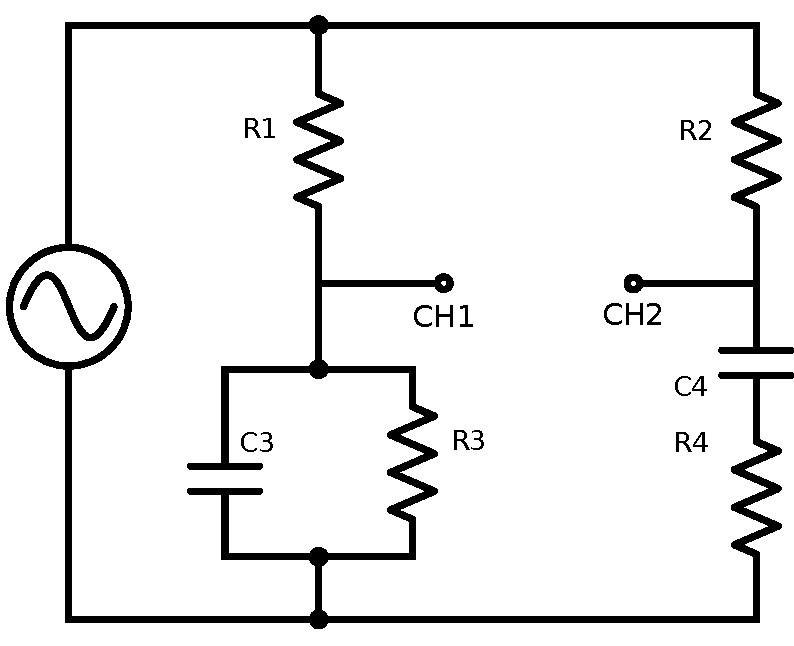
\includegraphics[width=0.30\textwidth]{schema1.pdf}
    \caption{Schema del circuito utilizzato per la misura di impedenza}
    \label{fig:circuito}
\end{wrapfigure}

\subsection{Acquisizione dati}
Una volta montato il circuito e collegato al generatore di forme d'onda sono stati collegati i due canali dell'oscilloscopio alle uscite del circuito (CH1 e CH2, come in Figura \ref{fig:circuito}). 
\`E stata fissata una tensione di $5\,Vpp$ e, dopo aver stabilizzato con il comando $trigger$ le forme d'onda sullo schermo e averle allineate, sono state impostate le funzioni integrate dell'oscilloscopio che permettevano di ricavare valori più stabili e meno affetti da rumore tramite la media di più misure.

Per calcolare il valore di capacità del condensatore incognito $C_3$ è stato necessario bilanciare il ponte. Ciò significa variare gli elementi circuitali, nel nostro caso $R_1$ (la decade di resistenze) e la frequenza $\omega$ a cui veniva generata la \emph{ddp} dal generatore finché i segnali che l'oscilloscopio leggeva da CH1 e CH2 fossero stati i medesimi.

Lavorando sulla frequenza e sulla resistenza abbiamo cercato quindi di bilanciare il circuito in modo tale che, in ogni momento, lo sfasamento tra CH1 e CH2 fosse nullo e l'ampiezza di segnale la stessa.

\subsection{Analisi dati}

La frequenza e la resistenza necessarie per bilanciare il ponte si sono rivelate essere:

\begin{equation*}
\omega \, = 2 \, \pi \, \nu \, = \, 2 \, \pi \, (2762.2 \pm 0.1) \, \si{\hertz}
\qquad R_1 \, = \, (14389 \pm 1) \, \si{\ohm}
\end{equation*}

\begin{equation}
\frac{R_4}{R_3} + \frac{C_3}{C_4} = \frac{R_2}{R_1}
\label{eq:1bilanciamento}
\end{equation}

\begin{equation}
\omega^2 \, R_3 \, C_3 \, R_4 \, C_4 \, = \, 1
\label{eq:2bilanciamento}
\end{equation}

da \ref{eq:1bilanciamento} e \ref{eq:2bilanciamento} si ottiene:

\begin{equation}
C_3 \, = \, \frac{C_4 \, R_2}{R_1 \, (1 \, + \, \omega^2 \, R_4^2 \, C_4^2)}
\end{equation}